\chapter{Secret Key Cryptography}

\section{Introduzione}
La crittografia a chiave segreta richiede l’uso di UNA sola chiave: dato un messaggio (il testo in chiaro) e la chiave, la cifratura produce
dati non intellegibili (il testo cifrato). Il testo cifrato ha circa la stessa lunghezza di quello in chiaro e la decifratura è l’inverso della cifratura, ed usa la stessa chiave. La crittografia a chiave segreta è talvolta chiamata crittografia \textbf{convenzionale} o crittografia \textbf{simmetrica}.
\begin{figure}[htbp]
	\centering%
	\subfigure%
	{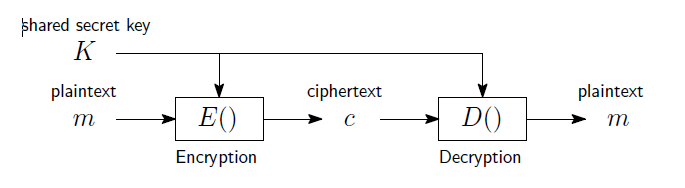
\includegraphics[height=13cm, width=13cm, keepaspectratio]{Immagini/Capitolo2/segreta_schema_blocchi.png}}
	\caption{Schema a blocchi crittografia a chiave segreta \label{fig:segreta_schema_blocchi}} 	
\end{figure}

\subsection{Impieghi crittografia a chiave segreta}
La crittografia a chiave segreta è alla base di molti meccanismi di sicurezza, i suoi principali impieghi sono: 
\begin{itemize}
  \item protezione della \textbf{confidenzialità} (l'uso classico di queste tecniche è rappresentato dalle \textbf{comunicazioni su un canale insicuro}, uno degli usi più moderni invece dalla \textbf{memorizzazione sicura su supporto insicuro})
  \item protezione dell'\textbf{integrità}: tramite queste tecniche possono essere eseguiti test per rilevare eventuali modifiche non consentite.
  \item autenticazione: tramite l'implementazione di protocolli per verificare l'identità di persone e/o processi.
\end{itemize}

\subsubsection{Comunicazioni su un canale insicuro}
In molte circostanze, due entità devono comunicare attraverso un canale insicuro correndo il rischio di essere ascoltate da una terza parte. Questo contesto è molto comune: si pensi alle reti LAN, che trasmettono dati in broadcast. La crittografia a chiave segreta permette a due entità che condividono un segreto (la chiave) di comunicare attraverso un canale insicuro, ove non può essere garantita l’assenza di intercettazioni/ascoltatori (eavesdropper), avendo la garanzia che il contenuto della comunicazione rimarrà confidenziale.

\subsubsection{Memorizzazione sicura}
Si supponga di disporre di un supporto di memorizzazione non protetto (ad esempio accessibile a molti utenti). Se si desidera salvare i dati proteggendone la confidenzialità si può definire una chiave segreta, salvare i dati dopo averli crittografati con tale chiave e custodire la chiave segreta in un luogo protetto. Il rischio dell'uso di questa tecnica consiste nella possibilità di smarrimento della chiave. In tal caso i dati sarebbero irrevocabilmente persi.

\subsubsection{Autenticazione forte}
Per \textbf{autenticazione forte (strong authentication)} si intende che si è in grado di provare la conoscenza di un segreto, che contraddistingue l’identità di una data entità, senza rivelarlo. L’autenticazione forte è ottenibile utilizzando la crittografia a chiave segreta, ed è particolarmente utile quando due processi devono comunicare su uba rete insicura. A rigore il segreto che contraddistingue l'identitò che si desidera autenticare dovrebbe essere noto solo a quest'ultima. Nella crittografia chiave segreta tale requisito non piò essere soddisfatto. Il segreto in questione è una chiave crittografica che deve essere nota anche all'entità autenticante.

\subsubsection{Esempio}
Si supponga che Alice e Bob condividano una chiave segreta $K_{AB}$ e che vogliano autenticarsi reciprocamente, cioè ciascuno vuole accertarsi dell'identità dell'altro. \newline \textbf{ipotesi:} $K_{AB}$ è nota solo ad Alice e Bob. Alice deve dimostrare a Bob di conoscere $K_{AB}$ senza rivelarla e viceversa. \newline \textbf{Strategia a sfida e risposta:} ciascuno dimostra di conoscere $K_{AB}$ rispondendo ad una sfida posta dall'altro. La \textbf{sfida} è un numero/stringa random \textbf{r} non prevedibile e sempre diversa. La \textbf{risposta} alla sfida è la sfida stessa cifrata \textbf{$E(K_{AB},R)$}. In \figurename ~\ref{fig:strong_auth_sec} è riportato un possibile schema di autenticazione a sfida e risposta (challenge-response) a chiave segreta. La procedura segue i seguenti passi:
\begin{itemize}
  \item Alice genera un numero random $r_{A}$ (la sfida) e la invia al presunto Bob
  \item il presunto Bob critta la sfida con la sua chiave segreta $K'_{AB}$ e restituisce ad Alice la risposta $E(K'_{AB}, r_{A})$
  \item Alice riceve la risposta del presunto Bob e la decritta con la chiave $K_{AB}$, cioè calcola $D(K_{AB},E(K'_{AB}, r_{A}))$. Se ottiene $r_{A}$, allora il presunto Bob è realmente Bob poiché con elevatissima probabilità, se $D(K_{AB},E(K'_{AB}, r_{A})) = r_{A}$, allora $K'_{AB} = K_{AB}$. In caso negativo deduce invece che il presunto Bob è un impostore. In modo analogo Bob verifica l'identità di Alice.
\end{itemize}
\begin{figure}[htbp]
	\centering%
	\subfigure%
	{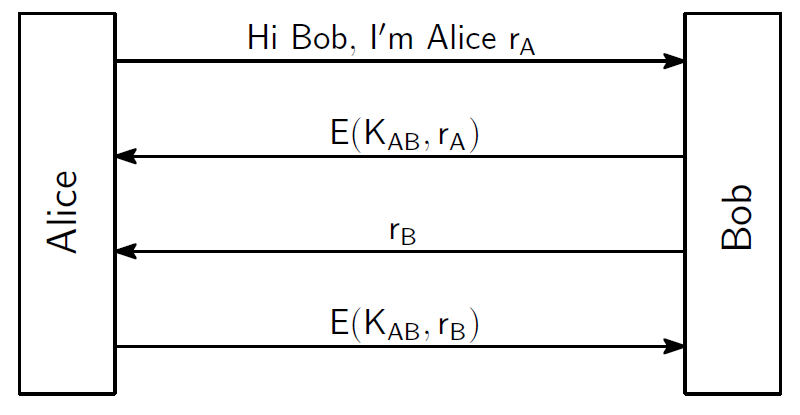
\includegraphics[height=13cm, width=13cm, keepaspectratio]{Immagini/Capitolo2/strong_auth_secret.png}}
	\caption{Schema a blocchi crittografia a chiave segreta \label{fig:strong_auth_sec}} 	
\end{figure}
La sicurezza del precedente protocollo si fonda sulle seguenti condizioni che non devono venire meno:
\begin{itemize}
  \item solo e soltanto Alice e Bob devono conoscere la chiave segreta $K_{AB}$
  \item le sfide generate devono essere \textbf{randomiche}, e di conseguenza non prevedibili, e \textbf{non ripetibili}, cioè la probabilità che due sfide si ripetano deve tendere a zero. L'attaccante potrebbe infatti collezionare molte coppie testo in chiaro/testo cifrato.
  \item è importante quindi che il numero di bit di una sfida sia superiore ad una data soglia (almeno 64 bit)
\end{itemize}

\subsubsection{Controllo di integrità}
La verifica dell’integrità di un messaggio inviato o di un file è un problema ricorrente in telecomunicazioni e in informatica. Per rilevare eventuali modifiche accidentali si fa uso generalmente di codici (somme) di controllo, detti anche \textbf{checksum}. Un \textbf{checksum} associa ad un qualsiasi messaggio $\textbf{m} \in \{0,1\}^*$ un codice di lunghezza prefissato di $b$ bit (generalmente $b = 32,64,128$ bit): $ck(\textbf{m}) \in \{0,1\}^b$. Un buon \textbf{checksum} dovrebbe variare in modo significativo anche a fronte di iminime variazioni dell'input. \newline \newline 
La sorgente del messaggio $m_{s}$ rende pubblico/invia il corrispondente checksum $ck(m_{s})$. Chi riceve il messaggio $m_{r}$ calcola il checksum e verifica se vale l'uguaglianza $ck(m_{s}) = ck(m_{r})$. In caso affermativo, conclude che $m_{s} = m_{r}$. Si noti tuttavia che, seppur improbabile, è possibile ottenere dei falsi positivi, cioè $ck(m_{s}) = ck(m_{r} )$ anche se non è vero.

\subsubsection{Checksum segreti e non segreti}
I codici di controllo servono per proteggere l’hardware da difetti e da inevitabili errori/guasti. Esistono codici di controllo molto sofisticati come i \textbf{CRC (Cyclic Redundancy Check)} per i quali la probabilità di falsi positivi è estremamente ridotta. Esistono anche i codici \textbf{FEC (Forward Error Correction)} che permettono di correggere eventuali errori oltre che a rilevarli (aggiungendo ulteriore ridondanza). Tuttavia entrambe queste tecniche \textbf{non} sono utilizzabili per la protezione contro attacchi intelligenti. Essendo pubblici, infatti, un avversario intelligente che vuole cambiare un messagio potrebbe modificare anche il codice di controllo in maniera coerente.\newline \newline
Per la protezione contro modifiche maliziose ad un messaggio, è richiesto un codice di controllo (checksum) segreto. Se l'algoritmo non è noto, nessuno può calcolare il checksum corretto per il messaggio modificato. Chiaramente, come nel caso degli algoritmi di cifratura, anziché un
algoritmo segreto conviene avere un algoritmo noto a tutti che richiede la conoscenza di una chiave segreta per il calcolo di un codice di controllo (Vedi pagina ~\pageref{sec:openStruct}, principio \textbf{Open Structure}). \newline \newline
In ciò consiste appunto un checksum cifrato, detto anche \textbf{MIC (Message Integrity Code)}. Il funzionamento del MIC è il seguente:
\begin{itemize}
  \item l'algoritmo produce un codice di autenticazione di lunghezza fissa $MIC(K,m)$, denominato anche \textbf{MAC (Message Authentication Code)}
  \item il codice MIC MIC(K,m) viene trasmesso insieme al messaggio m stesso
  \item formalmente l’input è una coppia $(K,m) \in \{0, 1\}^k \times \{0, 1\}^*$, dove $k$ denota il numero di bit della chiave segreta K, mentre l'output è sempre una stringa binaria di lunghezza prefissata, cioè $MIC(K,m) \in \{0, 1\}^b$
\end{itemize}

\subsection{Cifrari a blocchi e cifrari a flusso}
Un \textbf{cifrario a blocchi} elabora un blocco di elementi in ingresso per volta, producendo un blocco di uscita per ciascun blocco di ingresso. Questa metodologia implica quindi che:
\begin{itemize}
  \item il testo in chiaro deve essere preliminarmente suddiviso in blocchi
  \item il testo cifrato si ottiene combinando i vari blocchi cifrati
\end{itemize}
DES, IDEA e AES sono esempi di cifrari a blocchi simmetrici. Un \textbf{cifrario a flusso}, invece, elabora continuamente gli elementi in ingresso, producendo in uscita un "flusso" di elementi cifrati. Gli elementi cifrati vengono prodotti singolarmente, uno alla volta, man mano che la cifratura procede.

\section{Cifratura a blocchi}

\subsection{Introduzione e concetti generali}
L’algoritmo di cifratura converte un blocco di testo in chiaro in un blocco di testo cifrato. La chiave K non deve essere troppo corta (e.g. se K ha lunghezza 4 bit, sono sufficienti $2^4 = 16$ tentativi per individuarla). Analogamente la lunghezza (fissata) di un blocco non deve essere troppo piccola (e.g. se un blocco ha lunghezza 8 bit, ottenendo delle coppie plaintext - ciphertext si potrebbe costruire una tabella di $2^8 = 256$ coppie utilizzabile per la decfiratura).\newline 
D'altra parte, avere blocchi esageratamente lunghi oltre a non essere necessario dal punto di vista della sicurezza, comporta una gestione più complicata e può degradare le prestazioni. \textbf{64 bit è una lunghezza ragionevole per un blocco}: 
\begin{itemize}
  \item è improbabile ottenere ordine di $2^{64}$ coppie $\langle plaintext, ciphertext \rangle$ per costruire una tabella di decifratura, e
  \item anche se fosse possibile, la sua memorizzazione richiederebbe una spazio enorme ($2^{64}$ record da 64 bit),
  \item come pure l’ordinamento per consentire ricerche efficienti
\end{itemize}

